\documentclass[letter,12pt]{article}
\usepackage[paperheight=27.94cm,paperwidth=21.59cm,bindingoffset=0in,left=3cm,right=2.0cm, top=3.5cm,bottom=2.5cm, headheight=200pt, headsep=1.0\baselineskip]{geometry}
\usepackage{graphicx,lastpage}
\usepackage{upgreek}
\usepackage{censor}
\usepackage[spanish,es-tabla]{babel}
\usepackage{pdfpages}
\usepackage{tabularx}
\usepackage{adjustbox}
\usepackage{xcolor}
\usepackage{colortbl}
\usepackage{rotating}
\usepackage{multirow}
\usepackage[utf8]{inputenc}
\usepackage{float}

\renewcommand{\tablename}{Tabla}
\usepackage{fancyhdr}
\pagestyle{fancy}


%
\begin{document}
%
   \title{\Huge{Informe Laboratorio 1}}

   \author{\textbf{Sección 1} \\  \\Alumno 1 \\ e-mail: alumno.contacto@mail.udp.cl}
          
   \date{Agosto de 2024}

   \maketitle
   
   \tableofcontents
 
  \newpage
  

\section{Descripción}

\begin{enumerate}
    \item  Usted empieza a trabajar en una empresa tecnológica que se jacta de poseer sistemas que permiten identificar filtraciones de información a través de Deep Packet Inspection (DPI).
    A usted le han encomendado auditar si efectivamente estos sistemas son capaces de detectar las filtraciones a través de tráfico de red. Debido a que el programa ping es ampliamente utilizado desde dentro y hacia fuera de la empresa, su tarea será crear un software que permita replicar tráfico generado por el programa ping con su configuración por defecto, pero con fragmentos de información confidencial. Recuerde que al comparar tráfico real con el generado no debe gatillar alarmas.
    De todas formas, deberá hacer una prueba de concepto, en la cual se demuestre que al conocer el algoritmo, será fácil determinar el mensaje en claro.
    Para los pasos 1,2,3 indicar el texto entregado a IA Generativa y validar si el código resultante cumple con lo requerido.


\end{enumerate}


\section{Actividades}


\subsection{Algoritmo de cifrado}

\begin{enumerate}
\item Generar un programa, en python3 utilizando IA Generativa, que permita cifrar texto utilizando el algoritmo Cesar. Como parámetros de su programa deberá ingresar el string a cifrar y luego el desplazamiento.
\begin{figure}[H]
        \centering
        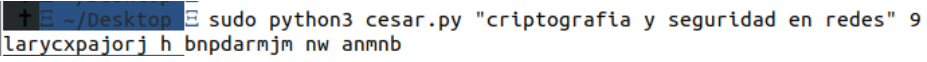
\includegraphics[width=15cm]{actividades/A1.png}
        \label{fig:a1}
\end{figure}


\end{enumerate}

\subsection{Modo stealth}

\begin{enumerate}
    \item Generar un programa, en python3 utilizando IA Generativa, que permita enviar los caracteres del string (el del paso 1) en varios paquetes ICMP request (un caracter por paquete en el campo data de ICMP) para de esta forma no gatillar sospechas sobre la filtración de datos.
Deberá mostrar los campos de un ping real previo y posterior al suyo y demostrar que su tráfico consideró todos los aspectos para pasar desapercibido.
    \begin{figure}[H]
        \centering
        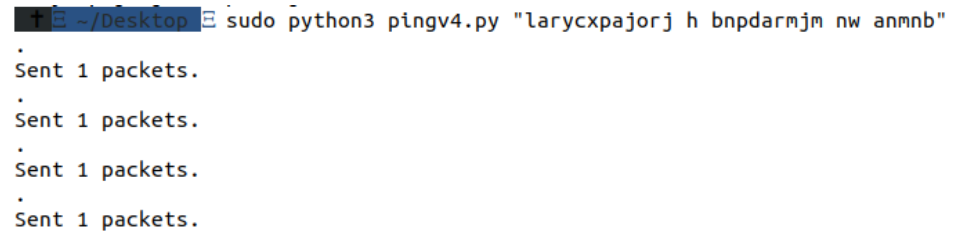
\includegraphics[width=15cm]{actividades/A2.1.png}
        \label{fig:a2-1}
    \end{figure}
    El último carácter del mensaje se transmite como una b.
    \begin{figure}[H]
            \centering
            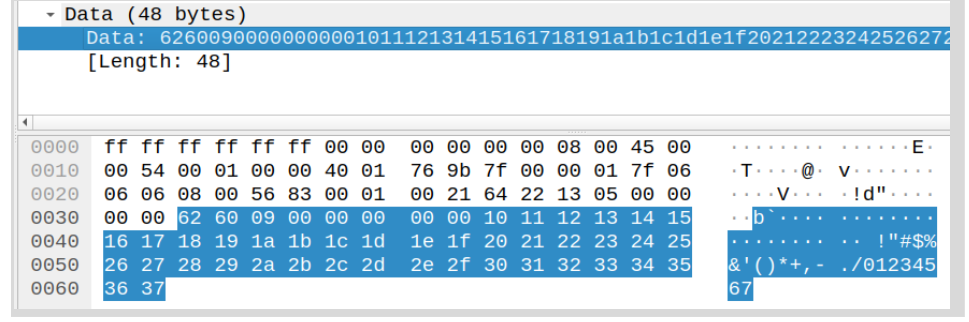
\includegraphics[width=15cm]{actividades/A2.2.png}
            \label{fig:a2-2}
        \end{figure}
\end{enumerate}

\subsection{MitM}
\begin{enumerate}
    \item Generar un programa, en python3 utilizando IA Generativa, que permita obtener el mensaje transmitido en el paso2. Como no se sabe cual es el desplazamiento utilizado, genere todas las combinaciones posibles e imprímalas, indicando en verde la opción más probable de ser el mensaje en claro.
    \begin{figure}[H]
        \centering
        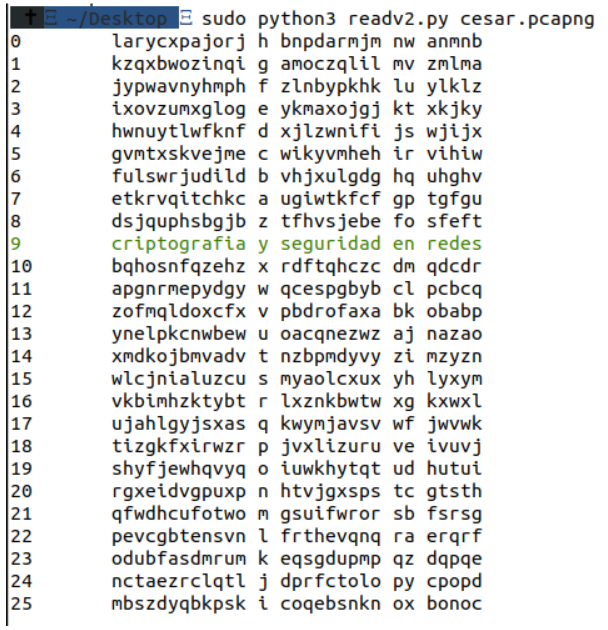
\includegraphics[width=12cm]{actividades/A3.png}
        \label{fig:a3}
    \end{figure}
    Finalmente, deberá indicar por que eligió esa IA Generativa en relación a otras del mercado. Comente si tuvo algún problema al momento de generar los códigos.

\end{enumerate}

\section{Desarrollo de Actividades}

\subsection{Actividad 1}

\subsection{Actividad 2}

\subsection{Actividad 3}


% Please add the following required packages to your document preamble:
%\begin{table}[htbp]

\section*{Conclusiones y comentarios}

\end{document}
